\chapter{Complex Relative Permittivity}

In the ground wave theory the complex relative permittivity is needed. This can be found in different ways\citep{Kim}. One of the easier ways to do this is the method described in \citep{Kim}. This method sets far less restrictions for the antennas compared to other methods\citep{Kim}. 

The theory behind the method comes from the the two-ray path loss model. A generic illustration of a two-ray setup can be seen in \autoref{fig:setup}.

\begin{figure}[H]
\centering
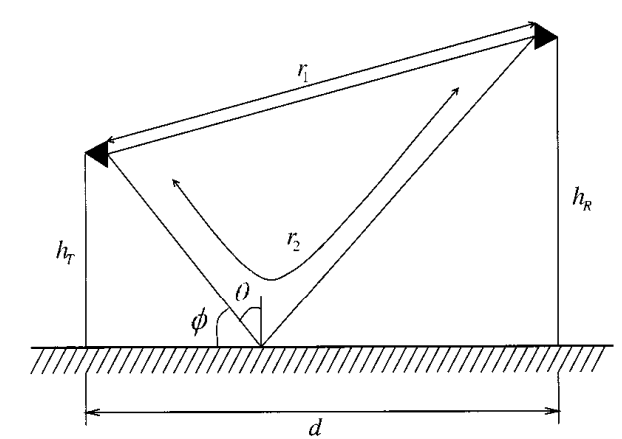
\includegraphics[width=0.6\textwidth]{figure/setup.png}
\caption{Illustration of setup and symbol meaning. Figure taken from \citep{Kim}.}
\label{fig:setup}
\end{figure}


The two-ray model can be written as\citep{Kim}:
\begin{equation}\label{two-ray}
P_r=\frac{P_tG_tG_t}{L}\left(\frac{\lambda}{4\pi}\right)^2\cdot\left|\frac{1}{r_1}\text{e}^{-jkr_1}+\sqrt{\alpha_t}\sqrt{\alpha_r}\rho_{h,v}\frac{1}{r_2}\text{e}^{-jkr_2}\right|^2
\end{equation}
\begin{where}
\va{$P_r$}{is the received power}{W}
\va{$P_t$}{is the transmitted power}{W}
\va{$G_t$}{is the transmitters antenna gain}{1}
\va{$G_r$}{is the receiver antennas gain}{1}
\va{L}{is loss factor for the cables and connectors}{1}
\va{$\lambda$}{is the wavelength}{m}
\va{$r_1$}{is the direct path length}{m}
\va{k}{is the wavenumber}{$m^{-1}$}
\va{${\alpha_t}$}{is the magnitude ratios of power along the reflected to the direct path directions for the transmit antenna}{1}
\va{${\alpha_r}$}{is the magnitude ratios of power along the reflected to the direct path directions for the receiver antenna}{1}
\va{$\rho_{h,v}$}{is the reflection coefficient in for either horizontal or vertical polarization}{1}\\
\va{$r_2$}{is the reflected path length}{m}
\end{where}

Do note that if the signal measured was horizontal polarized the horizontal reflection coefficient is used, if vertical polarized then the vertical reflection coefficient is used.

Since the reflection coefficient is complex it can be utilized that

\begin{equation}\label{rho}
\rho_{h,v} = \Gamma_{h,v}+j\zeta_{h,v}
\end{equation}
\begin{where}
\va{$\Gamma_{h,v}$}{is the real part of the permittivity}{1}
\va{$\zeta$}{is the imaginary part of the permittivity}{1}
\end{where}

By using \autoref{rho} in \autoref{two-ray} and rearranging, it can be seen that this draws circles on the complex reflection coefficient plane:

\begin{equation}\label{two-ray-circle}
\left(\Gamma_{h,v}+\frac{r_r\cos(kr_d)}{\sqrt{\alpha_r}\sqrt{\alpha_t}}\right)^2+\left(\zeta_{h,v}+\frac{r_r\sin(kr_d)}{\sqrt{\alpha_r}\sqrt{\alpha_t}}\right)^2=\left(\frac{4\pi r_2 \sqrt{P_d}}{\lambda\sqrt{\alpha_r}\sqrt{\alpha_t}}\right)^2
\end{equation}
\begin{where}
\va{$r_r$}{is $\frac{r_2}{r_1}$}{1}
\va{$r_d$}{$r_2-r_1$}{m}
\va{$P_d$}{$\frac{P_rL}{P_tG_tG_r}$}{1}
\end{where}


Since this is a circle three separate measurements is needed to get a unique intersection point. Because the complex relative permittivity vary with frequency and incidence angle, these must be fixed for the measurements. This is illustrated in \autoref{fig:measurepoints}.

\begin{figure}[H]
\centering
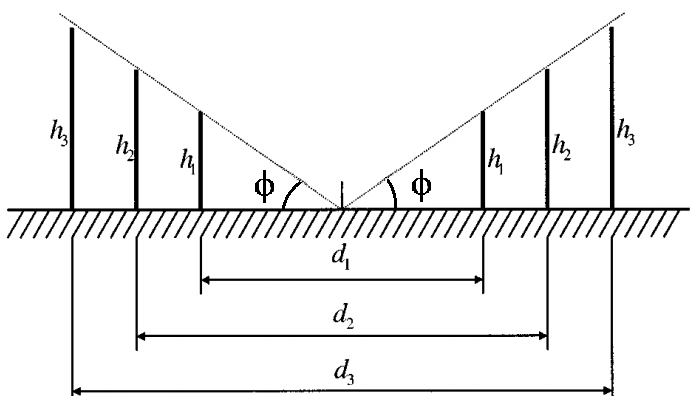
\includegraphics[width=0.6\textwidth]{figure/measurepoints.png}
\caption{Illustration of the three distances and heights needed. Figure taken from \citep{Kim}.}
\label{fig:measurepoints}
\end{figure}

When the intersection point has been determined\footnote{In practice there might not be a unique solution, due to measurement inaccuracies, There will then be three intersections that are close, and a sufficient estimate can be found by averaging these \citep{Kim}.} for both horizontal and vertical polarized waves the complex relative permittivity can be found as\citep{Kim}

\begin{equation}\label{crp}
\epsilon_0=\epsilon-j60\sigma\lambda=\frac{(1+\rho_v)(1-\rho_h)}{1+\rho_h)(1-\rho_v)}
\end{equation}
\begin{where}
\va{$\epsilon_0$}{is the complex relative permittivity}{1}
\va{$\epsilon$}{is the dielectric constant of the ground relative to unity
in free space}{1}
\va{$\sigma$}{is the conductivity of the ground in mhos per meter}{$\frac{mhos}{m}$}
\end{where}

A stepwise procedure could then be:
\begin{enumerate}
	\item Decide frequency and incidence angle
	\item Decide measurement setup, including $P_t$ heights and distances between transmitter and receiver for all three measurements points
	\item Determine $G_t$, $G_r$, $L$, $\alpha_t$, $\alpha_r$ for both horizontal and vertical cases
	\item Calculate $\lambda$, k, $r_1$, $r_2$
	\item Measure $P_r$ in all six cases
	\item Find intersection point using \autoref{two-ray-circle} for both horizontal and vertical polarization
	\item Calculate the complex relative permittivity using \autoref{crp}
\end{enumerate}


